\chapter{Introduction}
\label{chap:introduction}

\section{Overview on Cloud computing}

Nowadays software isn't just installed on an arbitrary computer for a specific user who can fulfil his given requirements by solving a task with it. Quite the contrary is the case as the significance of software has increased dramatically throughout any kind of business sector. The demand on software products these days is immense and therefore also the complexity and variety has experienced a huge growth over the last decade. Many years ago the Internet built up the fundament of accessing and sharing information worldwide and today applications and services, relying on complex and huge software ecosystems, give people around the globe the opportunity to use them any time and anywhere they want to satisfy their needs. To make this work this obviously needs a lot of resources accessible in the global network. 

Here the famous and hyped term "Cloud computing", which describes the process of moving application and services to the internet (due to the schematic metaphor also denotes as "cloud"), comes into play. \cite{Dialogic_Corporation} In such intensive businesses with rare resources as we have it nowadays people have to concentrate on their specific tasks to be as productive, competitive and flexible as possible. Cloud computing supports this by providing a pool of resources allowing for sharing and scalable deployment of services, as needed, from almost any location, and for which the customer can be billed based on actual usage. \cite{Dialogic_Corporation}

How these resources are provided and shared depends on the specific requirements and can vary. Due to the common patterns of usages some different cloud types describing the strategy have established over time. \cite{Dialogic_Corporation}
\begin{itemize}
	\item \textbf{Private Cloud}: The sharing of resources stays in-house and a specific organization is responsible for operating and maintaining the cloud infrastructure.
	\item \textbf{Community Cloud}: Several organizations having a common interest operate and maintain the shared cloud infrastructure. For the participating organizations such a solution can be very cheap if they agree on the community model.
	\item \textbf{Public Cloud}: An organization renting the cloud infrastructure from a specific provider who is responsible for it. The infrastructure is publicly available on a commerical basis. 
	\item \textbf{Hybrid Cloud}: This is a mixture of the other existing types which can be tailored based on the concrete requirements for optimizing productivity. This can be for instance used if some data should be necessarily kept in-house and the rest could be outsourced in a Public Cloud.
	\end{itemize} 

Over the years different service models depending on the type of the provided resource have been established. 
Bascially they can be divided into three different types organized in a cloud computing stack with increasing abstraction level bottom-up.

\begin{figure}[h!]
	\centering
		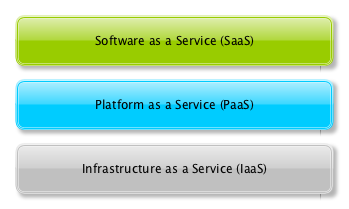
\includegraphics[width=0.75\textwidth]{service_models_stack}
	\caption{Stack of service models}
\end{figure}

\textbf{IaaS} basically means providing a shared pool of compute, storage and networking resources to end-users on a self-service basis. \cite{Oracle} This should help the end-users avoiding additional costs by buying dedicated hardware and setting up the instances to run their applications. They can easily manage and control the systems, in terms of operating system, network connectivity and storage and applications running on these instances but do not have to care about controlling and maintaining the cloud infrastructure. \cite{Dialogic_Corporation}

\textbf{PaaS} as the name already indicates provides the whole platform "out-of-the-box" to the end-user. This includes things like the operating system or network connectivity which are completely managed by the provider. The user only has to deploy her applications to the cloud. \cite{Dialogic_Corporation}

\textbf{SaaS} abstracts the platform and infrastructure and serves the software living in the cloud as a usable service to the end-user. \cite {Dialogic_Corporation}  This gives users instant access to such software without any special requirements such as downloading or installing and enables cross-platform as well as cross-device possibility. 